\subsubsection{ส่วนประกอบของหุ่นยนต์ฮิวมานอยด์}
\begin{figure}[ht]
	\centering
	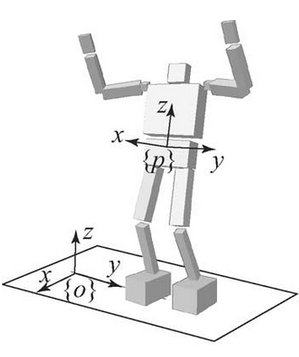
\includegraphics[width=0.4\textwidth]{chapter2/images/robot_component.png}
	\caption{ส่วนประกอบของหุ่นยนต์ฮิวมานอยด์}
	\label{fig:robot_component}
\end{figure}
หุ่นยนต์ฮิวมานอยด์ประกอบด้วยก้านต่อหลายๆก้านที่นำมาต่อกัน ลักษณะโครงสร้างนั้นจะเป็นแบบโซ่เปิด (Open kinematic chain)
และแต่ละก้านต่อจะเชื่อมต่อกันด้วยข้อต่อแบบหมุน เราสามารถแบ่งโครงสร้างของหุ่นยนต์ฮิวมานอยด์ออกเป็นส่วนหลักๆเป็น 2 ส่วน ส่วนแรกคือ
ส่วนก้านต่อของลำตัวหุ่นยนต์ (Torso) ซึ่งเราสามารถที่จะรวมไปถึงส่วนแขนกับหัวด้วย
และในส่วนที่สองคือ ส่วนก้านต่อของขาหุ่นยนต์ (Legs) ซึ่งเป็นส่วนขาของหุ่นยนต์ทั้งสองข้างที่สามารถนำไปที่สัมผัสกับพื้นได้
ทั้งสองก้านต่อนี้ถูกเชื่อมต่อกันด้วยส่วนของสะโพก (Hip) ที่อยู่ระหว่างส่วนลำตัวกับส่วนของขาหุ่นยนต์ ดังรูปที่ \ref{fig:robot_component}

\subsubsection{วัฏจักรการเดินของหุ่นยนต์ฮิวมานอยด์}
วัฏจักรการเดินของหุ่นยนต์ คือ การที่หุ่นยนต์จะต้องมีการถ่ายน้ำหนักไปมาระหว่างเท้าซ้ายและเท้าขวา
มีบางช่วงที่น้ำหนักตกลงบนเท้าข้างใดข้างหนึ่งหรือทั้งสองข้างพร้อมกัน สามารถแบ่งออกเป็นช่วงได้สองช่วง คือช่วงการยืนด้วยขาข้างเดียว
และช่วงการยืนด้วยขาทั้งสองข้าง
\begin{figure}[!ht]
	\centering
	\begin{subfigure}[b]{0.22\textwidth}
		\centering
		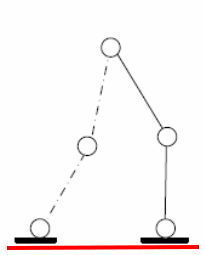
\includegraphics[width=\textwidth]{chapter2/images/doublesupport.png}
		\caption{ยืนด้วยขาสองข้าง}
		\label{fig:robot_walk_1}
	\end{subfigure}
	\hfill
	\begin{subfigure}[b]{0.45\textwidth}
		\centering
		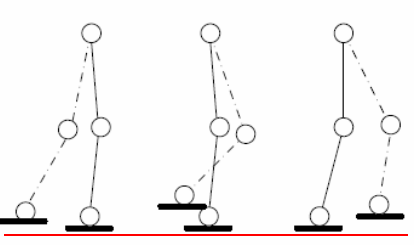
\includegraphics[width=\textwidth]{chapter2/images/singlesupport.png}
		\caption{ยืนด้วยขาข้างเดียว}
		\label{fig:robot_walk_2}
	\end{subfigure}
	\hfill
	\begin{subfigure}[b]{0.22\textwidth}
		\centering
		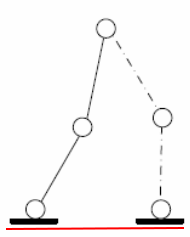
\includegraphics[width=\textwidth]{chapter2/images/doublesupport2.png}
		\caption{ยืนด้วยขาสองข้าง}
		\label{fig:robot_walk_3}
	\end{subfigure}
	\caption{วัฐจักรการเดินของหุ่นยนต์ฮิวมานอยด์}
	\label{fig:robot_walk_phase}
\end{figure}

\clearpage
\paragraph*{1) การยืนด้วยขาข้างเดียว :}
เป็นช่วงที่มีเท้าของหุ่นยนต์สัมผัสพื้นเพียงข้างเดียว ส่วนเท้าอีกข้างของหุ่นยนต์จะถูกยกลอยจากพื้น
โดยที่ไม่มีส่วนใดๆของขาข้างนั้นสัมผัสกับพื้นเลย ช่วงนี้จะเกิดขึ้นเมื่อมีการแกว่งเท้าจากข้างหลังไปข้างหน้า
ดังรูปที่ \ref{fig:robot_walk_2}

\paragraph*{2) การยืนด้วยขาสองข้าง :}
เป็นช่วงที่เท้าทั้งสองข้างของหุ่นยนต์สัมผัสกับพื้น ช่วงนี้จะเกิดตั้งแต่หุ่นยนต์วางเท้าขณะที่ส้นเท้าแตะกับพื้น
ไปจนถึง ปลายเท้าของขาอีกข้างหลุดออกจากพื้น

การเดินได้โดยไม่ล้มนั้น ตัวหุ่นยนต์จะต้องรักษาสมดุลของการเดินให้ได้ตลอดช่วงเวลาของการเดิน
ซึ่งสมดุลของการเดินแบบสองขาสามารถแบ่งตามลักษณะการเดินและการถ่ายน้ำหนักได้เป็น 2 รูปแบบหลัก คือ 
การเดินแบบสมดุลสถิต (static balance walking) และ การเดินแบบสมดุลพลวัต (dynamic balance walking)

\subsubsection{การสร้างและการควบคุมการเดินแบบสมดุลสถิต}
การเดินของหุ่นยนต์ในลักษณะนี้ จุดศูนย์กลางมวล (CoM) ของตัวหุ่นยนต์จะไม่มีการเคลื่อนไหวออกนอกบริเวณฐานรับน้ำหนัก (Supporting Area)
ตลอดช่วงเวลาการเดิน ไม่ว่าจะเป็นช่วงเวลาที่รับน้ำหนักด้วยเท้าข้างเดียวหรือทั้งสองข้างก็ตาม หมายความว่า โครงสร้างของหุ่นยนต์จะไม่ล้มแน่นอน
เนื่องจากการสร้างรูปแบบการเดินด้วยวิธีนี้จะควบคุมให้ตำแหน่งของจุดศูนย์กลางมวล อยู่ภายในพื้นที่ฐานรับน้ำหนักของหุ่นยนต์ตลอดเวลา
\ref{Legged robots walk the walk,https://blog.csiro.au/legged-robots-walk-walk/}

\begin{figure}[ht]
	\centering
	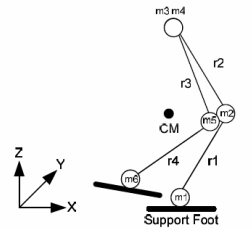
\includegraphics[width=0.4\textwidth]{chapter2/images/cominsupportpolygon.png}
	\caption{การควบคุมตำแหน่งของจุดรวมมวลให้อยู่ในพื้นที่ฐาน}
	\label{fig:robot_com_support}
\end{figure}

ข้อดีของการสร้างและควบคุมการเดินของหุ่นยนต์ด้วยวิธีนี้คือ สามารถสร้างรูปแบบการเดินได้โดยที่มีความซับซ้อนไม่มากนัก
สามารถสั่งให้หุ่นยนต์หยุดค้างในท่าทางใดๆก็ได้ตลอดเวลาโดยหุ่นยนต์ไม่ล้ม หุ่นยนต์ที่มีฝ่าเท้าใหญ่จะทำให้ง่ายต่อการก้าวเดินมากขึ้น
นอกจากการควบคุมการก้าวขาแล้วอาจเพิ่มการควบคุมส่วนลำตัวเพิ่มเติม เพื่อเป็นการเพิ่มเสถียรภาพในการเดินและการถ่ายเทน้ำหนัก
โดยที่อาจจะมีการเพิ่มเซนเซอร์วัดแรงที่ฝ่าเท้าเพื่อตรวจสอบการกระจายแรงกดที่ฝ่าเท้า เพื่อตรวจสอบว่าตำแหน่งของจุดรวมน้ำหนักอยู่บนพื้นที่ฝ่าเท้าหรือไม่
หรือเพื่อตรวจสอบเสถียรภาพของการเดินเพื่อแก้ไขท่าทางการเดินไม่ให้เกิดการล้ม

ข้อเสียของการควบคุมการเดินด้วยวิธีนี้คือ หุ่นยนต์จะใช้เวลาในการก้าวเดินมาก ใช้พลังงานในการเดินมากกว่าการเดินแบบสมดุลพลวัต
และท่าทางที่ได้จะมีความแตกต่างจากท่าทางการเดินของมนุษย์

\subsubsection{การสร้างและการควบคุมการเดินแบบสมดุลพลวัต}
การสร้างรูปแบบการเดินและควบคุมการเดินในลักษณะนี้ท่าทางการเดินของหุ่นยนต์นั้นจะคล้ายกับการเดินของมนุษย์มากกว่าแบบสถิต
เนื่องจากมีหลักการในการสร้างท่าทางที่เหมือนกับการเดินของมนุษย์ซึ่งมีขั้นตอนดังนี้คือ เอียงตัวให้ล้มไปในทิศทางที่ต้องการเดิน
เมื่อเริ่มเกิดการล้มขึ้นหุ่นยนต์จะเปลี่ยนตำแหน่งการวางเท้าไปยังตำแหน่งใหม่ เพื่อปรับให้โครงสร้างเข้าสู่สภาวะสมดุลอีกครั้ง

โดยธรรมชาติแล้วมนุษย์มีการถ่ายน้ำหนักในขณะที่เคลื่อนที่หรือยืนอยู่กับที่เพื่อรักษาสมดุลของท่าทางนั้นไว้
แต่หากการถ่ายโอนน้ำหนักนั้นเกิดสภาวะไม่สมดุล ร่างกายจะปรับสภาพโดยการเคลื่อนตำแหน่งของเท้าซึ่งเป็นพื้นที่ฐานออกจากเดิมไปยังตำแหน่งใหม่
เพื่อรักษาสมดุลไว้ หลักการดังกล่าวถูกนำมาใช้กับการควบคุมการเดินของหุ่นยนต์ฮิวมานอยด์ ในขณะที่หุ่นยนต์กำลังเคลื่อนไหว
ผลจากแรงเฉื่อยของการเคลื่อนที่และผลจากแรงดึงดูดของโลกมีผลต่อการเพิ่มและลดความเร่งให้การเดินของหุ่นยนต์
แรงเหล่านี้เรียกว่าแรงเฉื่อยรวมของการเคลื่อนที่ และเมื่อเท้าหุ่นยนต์สัมผัสกับพื้นจะได้รับผลกระทบของแรงนี้ เรียกว่า
แรงปฏิกิริยาจากพื้น

การตัดกันระหว่างแรงปฏิกิริยาจากพื้นและแนวแรงเฉื่อยรวม ตำแหน่งนั้นหากทำให้โมเมนต์เท่ากับศูนย์
เรียกจุดตัดนี้ว่าจุดโมเมนต์ศูนย์ ($ZMP_{robot}$) และจุดที่แรงปฏิกิริยาลงสู่พื้นว่า จุดปฏิกิริยาพื้นฐาน 
ท่าทางการเดินของหุ่นยนต์จะถูกกำหนดและถูกส่งให้กับชุดควบคุมข้อต่อจุดต่างๆของหุ่นยนต์ โดยให้สอดคล้องกับแรงเฉื่อยรวมที่เกิดขึ้นจากการคำนวณ
เรียกว่าแรงเฉื่อยรวมเป้าหมาย และจุดโมเมนต์ศูนย์ที่ได้จากการคำนวณเรียกว่าจุดโมเมนต์ศูนย์เป้าหมาย ($ZMP_{target}$)
เมื่อหุ่นยนต์เกิดสมดุลในขณะที่ทำการเดินได้อย่างสมบูรณ์ แนวแกนของแรงเฉื่อยรวมเป้าหมายและแรงปฏิกิริยาที่พื้นจะเป็นตำแหน่งเดียวกัน
แต่ในขณะที่หุ่นยนต์เดินผ่านพื้นผิวที่มีความขรุขระหรือไม่เรียบตำแหน่งสองจุดดังกล่าง จะไม่ใช่ตำแหน่งเดียวกันทำให้หุ่นยนต์เกิดการล้มได้
แรงที่ทำให้เกิดการล้มนี้เกิดจากตำแหน่งของจุดโมเมนต์ศูนย์และตำแหน่งแรงปฏิกิริยารวมที่พื้นไม่ตรงกัน ซึ่งเป็นสาเหตุหลักที่ทำให้เกิดความไม่สมดุลขึ้น
และเมื่อหุ่นยนต์เสียสมดุลระบบที่จะสามารถป้องกันการล้มและทำให้หุ่นยนต์เดินต่อไปได้อย่างต่อเนื่องคือ ระบบควบคุมแรงปฏิกิริยา
ระบบควบคุมจุดโมเมนต์ศูนย์ และระบบควบคุมการวางเท้า\ref{Achieving Stable walking,http://world.honda.com/ASIMO/history/technology2.html}

\begin{figure}[!ht]
	\centering
	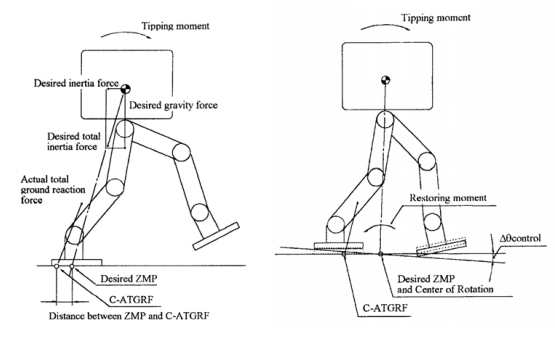
\includegraphics[width=0.7\textwidth]{chapter2/images/zmpdynamicwalking.png}
	\caption{การควบคุมตำแหน่งของจุดโมเมนต์ศูนย์ให้ตรงกับแรงปฏิกิริยารวม}
	\label{fig:robot_zmp_support}
\end{figure}

อย่างไรก็ตาม การสร้างท่าทางการเดินในลักษณะนี้ต้องใช้สมการในการคำนวณที่ซับซ้อนมาก
เนื่องจากต้องหาความสัมพันธ์ระหว่างองค์ประกอบหลายส่วน เช่น น้ำหนักของโครงสร้างในแต่ละส่วน 
แรงบิดที่แต่ละข้อต่อ และโมเมนต์โดยรวมของระบบ นอกจากนี้ยังต้องใช้อุปกรณ์การตรวจวัดต่างๆ เช่น เซนเซอร์วัดแรง
เซนเซอร์วัดมุม เซนเซอร์วัดแรงบิด ติดตั้งตามจุดต่างๆของโครงสร้างเพื่อวัดค่าออกมา ก่อนที่จะทำการคำนวณตำแหน่ง
และสร้างท่าทางการเดินของหุ่นยนต์ฮิวมานอยด์ ท่าทางการเดินที่ได้จากการควบคุมด้วยวิธีนี้ จะมีความคล้ายคลึงกับท่าทางการเดินของมนุษย์มาก

\subsubsection{จุดศูนย์กลางมวลของหุ่นยนต์}
หากต้องการให้หุ่นยนต์สามารถที่จะทรงตัวอยู่ได้โดยไม่ล้มนั้น จึงต้องรู้ตำแหน่งจุดศูนย์กลางมวลของหุ่นยนต์ตลอดเวลา
และต้องให้จุดศูนย์กลางมวลฉายตกในบริเวณฐานรับน้ำหนักของหุ่นยนต์โดยหาจากพื้นที่ที่ฝ่าเท้าสัมผัสกับพื้น
วิธีการนี้เป็นวิธีการทางสถิตศาสตร์